\documentclass[tikz,border=0pt,crop=true]{standalone}

\usepackage{tikz} % Allows creation of tikz pictures
\usepackage{varwidth}
\usetikzlibrary{arrows,shapes}

\begin{document}
    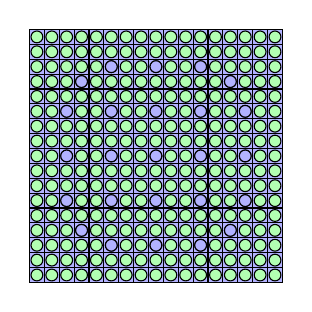
\begin{tikzpicture}[scale=0.15, every node/.style={scale=1}]
        \foreach \x in {0,1.26,...,20.16}
        \foreach \y in {0,1.26,...,20.16}
        \filldraw[xshift=\x cm, yshift=\y cm, fill=blue!30!white, 
        draw=black] (0, 0) rectangle (1.26,1.26) node[pos=.5] {};
        \foreach \x in {0,1.26,...,20.16}
        \foreach \y in {0,1.26,...,20.16}
        \filldraw[xshift=\x cm, yshift=\y cm, fill=green!30!white, 
        draw=black] (.63,.63) circle (.5) node[pos=.5] {};
        \foreach \x in {5*1.26, 8*1.26, 11*1.26}
        \foreach \y in {2*1.26, 14*1.26}
        \filldraw[xshift=\x cm, yshift=\y cm, fill=blue!30!white, 
        draw=black] (.63,.63) circle (.5) node[pos=.5] {};
        \foreach \x in {3*1.26, 13*1.26}
        \foreach \y in {3*1.26, 13*1.26}
        \filldraw[xshift=\x cm, yshift=\y cm, fill=blue!30!white, 
        draw=black] (.63,.63) circle (.5) node[pos=.5] {};
        \foreach \x in {2*1.26, 5*1.26, 8*1.26, 11*1.26, 14*1.26}
        \foreach \y in {5*1.26, 8*1.26, 11*1.26}
        \filldraw[xshift=\x cm, yshift=\y cm, fill=blue!30!white, 
        draw=black] (.63,.63) circle (.5) node[pos=.5] {};
    \end{tikzpicture}
\end{document}
